\clearpage
\VerdierPhysicalPageAnchor{0082}%
\VerdierSemanticAnchor{ch1-3}
\section{完全三角}

\VerdierSemanticAnchor{ch1-3-1}
\subsection{射の写像錐}

\VerdierSemanticAnchor{ch1-3-1-1}
\noindent\textbf{3.1.1.}\quad
\VerdierSemanticAnchor{ch1-3-1-1-tr1-category}
$C$ を加法圏とする。$\operatorname{tr}_1(C)$ により次の圏を表す：

\VerdierSemanticAnchor{ch1-3-1-1-objects}
\noindent--\quad $\operatorname{tr}_1(C)$ の対象は、$C$ の対象からなる複体の
（次数ゼロの）射 $X\xrightarrow{f}Y$ である。

\VerdierSemanticAnchor{ch1-3-1-1-morphisms}
\noindent--\quad $X\xrightarrow{f}Y$ と $X'\xrightarrow{f'}Y'$ を
$\operatorname{tr}_1(C)$ の二つの対象とする。$X\xrightarrow{f}Y$ から
$X'\xrightarrow{f'}Y'$ への射とは三つ組 $(g,h,a)$ であり、ここで
$g\colon X\longrightarrow X'$ と $h\colon Y\longrightarrow Y'$ は次数ゼロの
複体の射であり、
\VerdierSemanticAnchor{ch1-3-1-1-homotopy-data}
$a\colon f'g\rightsquigarrow hf$ は $f'g$ と $hf$ を結ぶホモトピーである。

\VerdierSemanticAnchor{ch1-3-1-1-composition}
\noindent--\quad
\begin{equation*}
  \begin{aligned}
    (g,h,a)\colon (X\xrightarrow{f}Y)
      &\longrightarrow (X'\xrightarrow{f'}Y'),\\
    (g',h',a')\colon (X'\xrightarrow{f'}Y')
      &\longrightarrow (X''\xrightarrow{f''}Y'')
  \end{aligned}
\end{equation*}
を $\operatorname{tr}_1(C)$ の二つの射とする。合成射
\begin{equation*}
  (g'',h'',a'')\colon
  (X\xrightarrow{f}Y)\longrightarrow(X''\xrightarrow{f''}Y'')
\end{equation*}
を次の等式で定める：

\VerdierSemanticAnchor{ch1-3-1-1-eq1}
\begin{equation}
  \begin{aligned}
    g''&=g'g,\\
    h''&=h'h,\\
    a''&=a'\star g+h'\star a.
  \end{aligned}
  \tag{3.1.1.1}
\end{equation}

\VerdierSemanticAnchor{ch1-3-1-1-category-verification}
このようにして確かに圏が定義されたことは直ちに確かめられる。
\VerdierSemanticAnchor{ch1-3-1-1-diagram-representation}
$\operatorname{tr}_1(C)$ の射
$(g,h,a)\colon(X\xrightarrow{f}Y)\longrightarrow(X'\xrightarrow{f'}Y')$
は、通常次の図で表す：

\VerdierSemanticAnchor{ch1-3-1-1-eq2}
\begin{equation}
  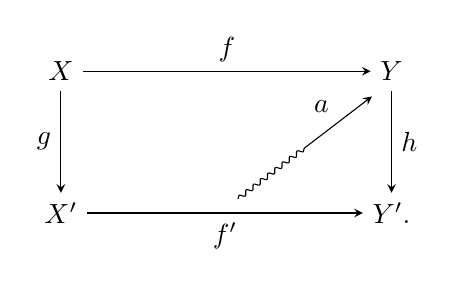
\begin{tikzpicture}[>=stealth,baseline=(current bounding box.center)]
    \node (X)  at (0,1.8) {$X$};
    \node (Y)  at (4.2,1.8) {$Y$};
    \node (Xp) at (0,0) {$X'$};
    \node (Yp) at (4.2,0) {$Y'\mathpunct{.}$};
    \draw[->] (X) -- node[above] {$f$} (Y);
    \draw[->] (X) -- node[left] {$g$} (Xp);
    \draw[->] (Y) -- node[right] {$h$} (Yp);
    \draw[->] (Xp) -- node[below] {$f'$} (Yp);
    \draw[decorate,decoration={snake,amplitude=0.8pt,segment length=3.3pt}]
      (2.25,0.18) -- (3.10,0.83);
    \draw[->] (3.10,0.83) -- node[above left] {$a$} (3.95,1.48);
  \end{tikzpicture}
  \tag{3.1.1.2}
\end{equation}
